\documentclass[12pt]{exam}

\usepackage{amssymb}
\usepackage{mathtools}
\usepackage{algorithm}
\usepackage{float}  % Figure placement
\usepackage{minted}  % Code highlighting
\usepackage{tikz}  % Flow chart
\usetikzlibrary{positioning, arrows.meta}
\usepackage{lipsum}
\usepackage{xspace}
\usepackage{hyperref}
\usepackage{MnSymbol}
\usepackage{pgffor}
\usepackage{colortbl}
\usepackage{multirow}
\usepackage{array}
\usepackage{enumitem}
\usepackage{multicol}
\usepackage{forest}



\hypersetup{
    colorlinks = true,
    linkcolor = blue,
    urlcolor  = blue,
    citecolor = blue,
    anchorcolor = blue
}

\newcommand{\hwheaderfooter}[3]{
\pagestyle{headandfoot}
\firstpageheadrule
\firstpageheader{#1}{#2}{#3}
\runningheader{#1}{#2}{#3}
\runningheadrule
\firstpagefooter{}{\thepage}{}
\runningfooter{}{\thepage}{}
}

\newcommand{\latex}{\LaTeX\xspace}

\newcommand{\stars}[1]{%
    \foreach \n in {1,...,#1}{%
        $\filledstar$%
    }%
}

\hwheaderfooter{HW 7}{Ching}{CSCI 406}


\begin{document}
\begin{center}
    \fbox{\fbox{\parbox{\textwidth - 0.2 in}{\centering

                {Instructions: Please note that handwritten assignments \textbf{will not be graded}. Use the
                    provided \latex template to complete your homework. Please do not alter the order or spacing of
                    questions (keep each question on its own page). When you submit to Gradescope, you must mark
                    which page(s) correspond to each question. \textbf{You may not receive credit for unmarked
                        questions}. \\ When including graphical figures, we encourage the use of tools such as \href{https://dreampuf.github.io/GraphvizOnline/}{graphviz} or packages like \href{https://www.overleaf.com/learn/latex/TikZ_package}{tikz} for simple and complex figures. However, these may be handwritten only if they are neat and legible (as defined by the grader). }
            }}}
\end{center}

\textbf{List any collaborators (besides TAs or professors) here:}

\begin{questions}

    \question[5] [W9, \stars{1}] For the following questions, select whether the statement is true or false.
    \textbf{No explanation is necessary for these problems.}

    \begin{parts}
        \part Dynamic programming is a technique to optimize certain types of recursive algorithms.\\
        $\blacksquare$ True $\square$ False

        \part Dynamic programming is a technique which increases time complexity in order to decrease space complexity.\\
        $\square$ True $\blacksquare$ False

        \part Dynamic programming can be applied to problems where there are multiple ways to arrive at the same subproblem instance via many branches of a recursion tree.\\
        $\blacksquare$ True $\square$ False

        \part When computing values in a dynamic programming table, we always start in the upper-left corner of the table.\\
        $\square$ True $\blacksquare$ False
    \end{parts}
    \clearpage

    \question[10] [W9, \stars{2}] DP Terminology. Consider the Fibonacci problem that was discussed in class. Match the following statements with the following terms.

    \begin{multicols}{2}
        \begin{enumerate}[label=(\Alph*)]
            \item Subproblem Instance
            \item Base Instance / Base Case
            \item Root Instance
            \item Recurrence Relation
            \item Recursive Algorithm
            \item Top-Down DP
            \item Bottom-Up DP
            \item Recursion Tree
            \item Computation DAG
        \end{enumerate}
    \end{multicols}

    \begin{parts}
        \part $\boxed{\text{Top-Down DP}}$ --- The following function:
        \begin{minted}{python}
    DP = {}
    def F(n):
        if n in DP: return DP[n]
        if f == 0: return 0
        if f == 1: return 1
        DP[n] = F(n-1) + F(n-2)
        return DP[n]
    \end{minted}
        \part $\boxed{\text{Root Instance}}$ --- Fibonacci of $n$
        \part $\boxed{\text{Recurrence Relation}}$ --- $F(n) = F(n-1) + F(n-2)$
        \part $\boxed{\text{Recursive Algorithm}}$ --- The following function:
        \begin{minted}{python}
    def F(n):
        if f == 0: return 0
        if f == 1: return 1
        return F(n-1) + F(n-2)
    \end{minted}
        \part $\boxed{\text{Computation DAG}}$ --- The following graph:

        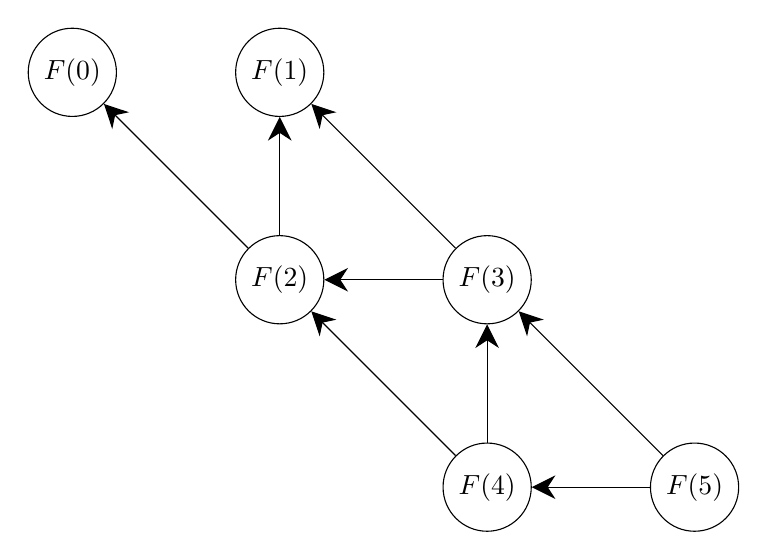
\begin{tikzpicture}[
            node distance = 1.5cm,
            circle/.style = {draw, shape=circle, minimum size=1cm},
            >=stealth,  % Set the arrow tip style
            line/.style = {draw, -{Stealth[length=3mm, width=3mm]}},
            ]
            \node[circle] (F0) {$F(0)$};
            \node[circle, right=of F0] (F1) {$F(1)$};
            \node[circle, below=of F1] (F2) {$F(2)$};
            \node[circle, right=of F2] (F3) {$F(3)$};
            \node[circle, below=of F3] (F4) {$F(4)$};
            \node[circle, right=of F4] (F5) {$F(5)$};

            \draw[line] (F2) -- (F1);
            \draw[line] (F2) -- (F0);
            \draw[line] (F3) -- (F2);
            \draw[line] (F3) -- (F1);
            \draw[line] (F4) -- (F3);
            \draw[line] (F4) -- (F2);
            \draw[line] (F5) -- (F4);
            \draw[line] (F5) -- (F3);
        \end{tikzpicture}
    \end{parts}
    \clearpage

    \question[5] [W9, \stars{3}] Binomial Coefficients. Select the true statement. \textbf{No explanation is necessary for this question.}

    In terms of $n$ and $k$, how many calls to the recursive algorithm are required to evaluate $\binom{n}{k}$?

    $\square$ $k^n$ \\
    $\square$ $n^k$ \\
    $\square$ $\binom{n}{k}$ \\
    $\blacksquare$ $2\binom{n}{k} - 1$ \\
    $\square$ $(n + k) k$
    \clearpage

    \question[40] [W9, \stars{5}] Stirling Numbers. This question is related to Wednesday's worksheet.

    Recall the definition of \textit{Stirling numbers of the second kind}:

    \textbf{Base Cases}
    \begin{align}
        S_{n,0} & = 0  & \forall n > 0 \\
        S_{n,k} & = 1  & n = k \ge 0   \\
        S_{n,1} & =  1 & \forall n > 1 \\
        S_{n,k} & = 0  & n < k
    \end{align}

    \textbf{General Case}
    \begin{align}
        S_{n,k} & = k \times S_{n-1,k} + S_{n-1,k-1}
    \end{align}

    \begin{parts}
        \part[15] Fill in the following \textbf{table} (starting with the base-cases).

        \begin{tabular}{ | r | r | r | r | r | r | r | r | r | } \hline
            $n / k$ & ~~0~~ & ~~1~~ & ~~2~~ & ~~3~~ & ~~4~~ & ~~5~~ & ~~6~~ & ~~7~~ \\ \hline
            0       & 1     & 0     & 0     & 0     & 0     & 0     & 0     & 0     \\ \hline
            1       & 0     & 1     & 0     & 0     & 0     & 0     & 0     & 0     \\ \hline
            2       & 0     & 1     & 1     & 0     & 0     & 0     & 0     & 0     \\ \hline
            3       & 0     & 1     & 3     & 1     & 0     & 0     & 0     & 0     \\ \hline
            4       & 0     & 1     & 7     & 6     & 1     & 0     & 0     & 0     \\ \hline
            5       & 0     & 1     & 15    & 25    & 10    & 1     & 0     & 0     \\ \hline
            6       & 0     & 1     & 31    & 90    & 65    & 15    & 1     & 0     \\ \hline
            7       & 0     & 1     & 63    & 301   & 350   & 140   & 21    & 1     \\ \hline
        \end{tabular}

        \part[10] Write an unoptimized \textbf{recursive algorithm} (no loops) to solve this problem in the programming language of your choice. Assume all necessary libraries/headers are present (only write the function). \textbf{Present your code using the minted \latex library. You shouldn't need more than 10 lines.}

        \begin{minted}{python}
        def stirling(n, k):
            # Base case 1 & 4
            if (k == 0 and n > 0) or (n < k):
                return 0
            # Base case 2 & 3
            elif (n == k and k >= 0) or (k == 1 and n > 1):
                return 1
            # General Case
            else:
                return (k * stirling(n-1, k)) + stirling(n-1, k-1)


    \end{minted}

        \part[5] Write a \textbf{``top-down'' DP solution} that augments the recursive algorithm above with memoization. Store intermediate results in a dictionary/array and check to see if a value has already been determined before computing it again. If the value has already been computed, then return it instead of making the recursive call(s).

        \begin{minted}{python}
        def sterling_top_down(n, k):
            # Create a dictionary to store the results
            S = {}
            # Base case 1 & 4
            if (k == 0 and n > 0) or (n < k):
                return 0
            # Base case 2 & 3
            elif (n == k and k >= 0) or (k == 1 and n > 1):
                return 1
            # General Case
            else:
                if (n, k) not in S:
                    S[(n, k)] = (k * sterling_top_down(n-1, k)) + \
                        sterling_top_down(n-1, k-1)
                return S[(n, k)]
    \end{minted}

        \part[10] Write a \textbf{``bottom-up'', iterative DP solution} that uses a \texttt{for} loop and an array to compute the solution starting from the base cases. Assume $n$ and $k$ have been previously provided to your program.

        \begin{minted}{python}
        def stirling_bottom_up(n, k):
            # Create a 2D array to store the results
            S = [[0 for _ in range(k+1)] for _ in range(n+1)]

            for row in range(n+1):
                # Base cases
                if k >= 1 and row > 1:
                    S[row][1] = 1
                if k >= row:
                    S[row][row] = 1

                # General Case
                if row >= 3 and k >= 2:
                    for col in range(2, min(row, k)+1):
                        S[row][col] = (col * S[row-1][col]) + S[row-1][col-1]

            return S[n][k]
    \end{minted}

    \end{parts}
    \clearpage

    \question[40] [W9, \stars{5}] Please present your code using the \texttt{minted} \latex library.

    You want to construct a rod of integer length $n$ using smaller rods. The smaller rods are available in three
    lengths: 1, 2, and 3 ft respectively. There are an unlimited number of these smaller rods available.
    Your plan is to glue several of the smaller rods end-to-end to create a longer rod.

    % \begin{figure}[H]
    %     \centering
    %     \includegraphics[width = 2 in]{Homeworks/theplank.png}
    %     \caption{There are 7 ways to make a 4 ft plank.}
    %     \label{fig:plank}
    % \end{figure}
    \begin{table}[H]
        \centering
        \begin{tabular}{|
                >{\columncolor[HTML]{00B050}}c cc
                >{\columncolor[HTML]{00B050}}c |}
            \hline
            \multicolumn{1}{|c|}{\cellcolor[HTML]{00B050}\textbf{1}} & \multicolumn{1}{c|}{\cellcolor[HTML] {00B050}\textbf{1}} & \multicolumn{1}{c|}{\cellcolor[HTML]{00B050}\textbf{1}} & \textbf{1} \\ \hline
            \multicolumn{1}{|c|}{\cellcolor[HTML]{00B050}\textbf{1}} & \multicolumn{1}{c|}{\cellcolor[HTML]{00B050}\textbf{1}}  & \multicolumn{2}{c|}{\cellcolor[HTML]{00B0F0}\textbf{2}}              \\ \hline
            \multicolumn{2}{|c|}{\cellcolor[HTML]{00B0F0}\textbf{2}} & \multicolumn{1}{c|}{\cellcolor[HTML]{00B050}\textbf{1}}  & \textbf{1}                                                           \\ \hline
            \multicolumn{1}{|c|}{\cellcolor[HTML]{00B050}\textbf{1}} & \multicolumn{2}{c|}{\cellcolor[HTML]{00B0F0}\textbf{2}}  & \textbf{1}                                                           \\ \hline
            \multicolumn{2}{|c|}{\cellcolor[HTML]{00B0F0}\textbf{2}} & \multicolumn{2}{c|}{\cellcolor[HTML]{00B0F0}\textbf{2}}                                                                         \\ \hline
            \multicolumn{1}{|c|}{\cellcolor[HTML]{00B050}\textbf{1}} & \multicolumn{3}{c|}{\cellcolor[HTML]{D60CBE}\textbf{3}}                                                                         \\ \hline
            \multicolumn{3}{|c|}{\cellcolor[HTML]{D60CBE}\textbf{3}} & \textbf{1}                                                                                                                      \\ \hline
        \end{tabular}
        \caption{Each of the 7 rows above gives us a different way to construct a 4 ft rod.}
    \end{table}

    Question: In how many ways can you glue the three types of smaller rods together to create a rod of length $n > 0$? The table above enumerates all of the possibilities when $n = 4$ and giving an answer of 7.

    \begin{parts}
        \part[5] What is the input to the \textbf{subproblem instance}?

        The input to the subproblem instance is the length of the rod, $n$.

        \part[5] Which subproblem instances are the \textbf{base cases}? What are their values?


        The base cases are when the length of the rod is 1, 2, or 3. Their values are 1, 2, and 4, respectively.

        \part[5] Develop notation and describe a \textbf{recurrence relation} between the subproblem instances.

        Let $W(n)$ be the number of ways to construct a rod of length $n$. Then, the recurrence relation is:
        \begin{align*}
            W(n) = W(n-1) + W(n-2) + W(n-3)
        \end{align*}


        \part[10] Write an unoptimized \textbf{recursive algorithm} (no loops) to solve this problem in the programming language of your choice. Assume all necessary libraries/headers are present (only write the function). \textbf{Present your code using the minted \latex library. You shouldn't need more than 10 lines.}
        \begin{minted}{python}
        def rod(n):
            # Base cases
            if n == 1:
                return 1
            if n == 2:
                return 2
            if n == 3:
                return 4
            # General Case
            return rod(n-1) + rod(n-2) + rod(n-3)
    \end{minted}

        \part[5] Draw the first three levels (the root is the first level) of the \textbf{recursion tree} for $n = 12$ and highlight the repeated computations, that is, identical recursive calls made more than once or \textbf{will} be made more than once if the tree was extended to further levels.

        \begin{forest}
            for tree={
            circle,
            draw,
            minimum size=2em,
            inner sep=1pt,
            s sep=10mm,
            },
            [12, name=root
            [11
                [10, fill=red!20]
                [9, fill=red!20]
                [8, fill=red!20]
            ]
            [10, fill=red!20
            [9, fill=red!20]
            [8, fill=red!20]
            [7, fill=red!20]
            ]
            [9, fill=red!20
            [8, fill=red!20]
            [7, fill=red!20]
            [6, fill=red!20]
            ]
            ]
        \end{forest}

        \part[10] Write a \textbf{``bottom-up'', iterative DP solution} that uses a \texttt{for} loop and an array to compute the solution starting from the base cases. Assume $n$ has been previously provided to your program.

        \begin{minted}{python}
        def rod_bottom_up(n):
            # Create an array to store the results
            W = [0] * (max(n+1,4))
            # Base cases
            W[1] = 1
            W[2] = 2
            W[3] = 4
            # General Case
            for i in range(4, n+1):
                W[i] = W[i-1] + W[i-2] + W[i-3]
            return W[n]
\end{minted}

    \end{parts}

    % close the document
\end{questions}
\end{document}